\chapterimage{back2.jpg} % Chapter heading image
\chapter{Clock}

This second project introduces the synchronous behaviour of the board. The outputs are updated regularly after a given period of time (a delay).\\
The equations that we would like to implement are:
\begin{center}
O$_1$ = not(O$_1$) every second (synchronous)\\
O$_2$ = not(O$_2$) all the time (asynchronous) 
\end{center}
O$_1$ changes its status every second between OFF and ON. 0$_2$ is the opposite of O$_1$: 0$_2$ is ON when O$_1$ is OFF, and OFF when O$_1$ is ON.

\section{Modelling}

The modelling requires three steps:
\begin{itemize}
    \item The first step is to create a project, to give it a name and select "CSSP project".
    \item The second step is to add a board (only one) and to change the names outputs to O1 and O2. Deselect the inputs as they are not going to be used in the following.
    \item The third step is to modify the components \textit{logic}, \textit{logic\_i}, \textit{user\_ctx} and \textit{user\_ctx\_i} to specify and implement the behaviour. 
\end{itemize}
 
 \lstset{frameround=fttt,keywordstyle=\color{ocre}\bfseries}
\lstinputlisting[language=B, frame=trbl, firstline=19,lastline=26,caption={Non-deterministic specification of the operation user\_logic},label=examples:clock1-spec, rulecolor=\color{ocre}]{chapterProjects/clock_1_logic.mch}

For \textit{logic}, we need to modify the specification of the operation user\_logic. We simply assert that the two outputs O1 and O2 are going to be modified non-deterministically such as  O1 and O2 are different (see listing \ref{examples:clock1-spec}). 

 \lstset{frameround=fttt,keywordstyle=\color{ocre}\bfseries}
\lstinputlisting[language=B, frame=trbl, firstline=5,lastline=10,caption={Declaration of the constant delta\_t in user\_ctx},label=examples:clock1-user-ctx, rulecolor=\color{ocre}]{chapterProjects/clock_1_user_ctx.mch}

We need to modify \textit{user\_ctx} to introduce a constant representing the duration of the delay expressed in milliseconds. This constants is named delta\_t; it is defined over 32 bits and is different from 0 (see listing \ref{examples:clock1-user-ctx}).

 \lstset{frameround=fttt,keywordstyle=\color{ocre}\bfseries}
\lstinputlisting[language=B, frame=trbl, firstline=9,lastline=11,caption={Valuation of the constant delta\_t in user\_ctx\_i},label=examples:clock1-user-ctx-i, rulecolor=\color{ocre}]{chapterProjects/clock_1_user_ctx_i.imp}

In \textit{user\_ctx\_i}, we provide a value for the constant deltat\_t that is compatible with the two constraints: delta\_t is a unsigned integer defined over 32 bits and is different from 0. We choose the value 1000 \footnote{Put for 1000 milliseconds.} (see listing \ref{examples:clock1-user-ctx-i}).

 \lstset{frameround=fttt,keywordstyle=\color{ocre}\bfseries}
\lstinputlisting[language=B, frame=trbl, firstline=24,lastline=47,caption={Operation user\_logic in user\_ctx\_i},label=examples:clock1-logic-i, rulecolor=\color{ocre}]{chapterProjects/clock_1_logic_i.imp}

For \textit{logic\_i}, We only need to modify the body of the operation user\_logic (see listing \ref{examples:clock1-logic-i}). \\
We need three local variables: ms\_tick\_cycle representing the number of milliseconds elapsed since the last reset, s\_tick\_cycle representing the number of times the delay has elapsed, and tick which represents the current state of the tick (OFF or ON). We define them with the substitution VAR ... IN ... END.  These three variables are typed prior to any use, by using the "becomes such that" substitution with the type uint32\_t.\\
The  number of milliseconds elapsed since the last reset is collected by calling the operation get\_ms\_tick. The number of times the delay has elapsed is computed by divided the number of milliseconds elapsed since the last reset by the duration of the delay deltat\_t. Finally the status of the tick (OFF or ON) is computed with a modulo 2 of the number of times the delay has elapsed. The output O1 is then set when tick is equal to 0 and reset when equals to 1. Finally O2 is computed with the last IF THEN ELSE, based on the value computed for O1.

\begin{remark}
Do not set the delay deltat\_t to a value less than 50 as very quick activation/deactivation of the output relays are going to kill them.
\end{remark}

\section{Executing}

Now that the modelling is complete, we first need to check and prove the model. Select all the components by clicking on the central pane of the main window\footnote{the one showing all the components of the project.}, then type ctrl+A. Type ctrl+0 to initiate the typecheck, proof obligation generation and proof of all these components. If some mistake was made, error messages are displayed either in the model editor or the error/warning pane in the main window. Be sure to correct any mistake before moving on. Finally press ctrl+U to complete the proof. You should obtain the proof status of the figure \ref{projects:Clock_1-project-status} (the Unproved column shows only zeros, meaning that the project is fully proved).

\begin{figure}[h]
\centering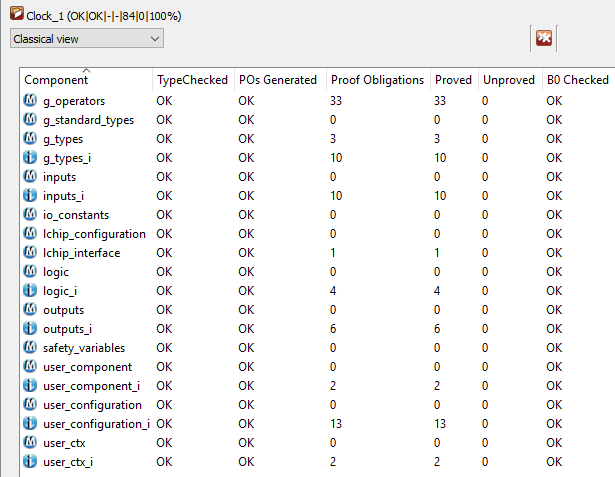
\includegraphics[scale=0.5]{Pictures/chaptProjects/clock1-project-status.png}
\caption{Clock\_1 project status}
\label{projects:Clock_1-project-status}
\end{figure}

The project is ready to be compiled. Be sure that your SK0 board is connected with the USB connector to your host. Right-click on the project name in the left pane and select "CSSP Runner". 
A new window appears, showing a carousel of all the steps of the compilation. Click on the green triangle on the top left. All steps are cleared until the last one where you are asked to reset the SK0 board. Use a pen to push on the reset button and release it. The board starts to blink as it enters bootload mode. After around 30s, the last step is cleared (green check) and you are again invited to reset the SK0 board. Push the reset button and release it. After 2 seconds, the board starts to execute your program.

\section{Testing}

To test your program, you just need to check that, when running, the behaviour is as expected: $0\_1$ beating every second and $0\_2$  is the opposite state of $0\_2$.

\begin{exercise}
Create a program which implements the following equations:
\begin{center}
O$_1$ = not(O$_1$) every second (synchronous)\\
O$_2$ = not(O$_2$) every 2.5 seconds (synchronous)  
\end{center}
First create a new project and populate it with models similar to Clock\_1. Add another constant delta\_t1 valued with 2500. Then modify the body of the operation user\_logic in the component \textit{logic\_i} to implement two clocks over the outputs $0\_1$ and $0\_2$ .
\end{exercise}